\documentclass[aspectratio=169,11pt]{beamer}
\usetheme{Madrid}
\usecolortheme{seahorse}

\usepackage[english]{babel}
\usepackage{fontspec}
\usepackage{amsmath}
\usepackage{booktabs}
\usepackage{graphicx}
\usepackage{xcolor}
\usepackage{adjustbox}

\title{Project of Econometrics}
\author{Greco Hernández \and Rachel Martínez Guerrero}
\institute{Anime Research}
\date{\today}

\setbeamertemplate{navigation symbols}{}
\setbeamertemplate{footline}{
  \leavevmode
  \hbox{
    \begin{beamercolorbox}[wd=.79\paperwidth,ht=2.5ex,dp=1ex,leftskip=1em]{author in head/foot}
      Greco Hernández \& Rachel Guerrero
    \end{beamercolorbox}
    \begin{beamercolorbox}[wd=.19\paperwidth,ht=2.5ex,dp=1ex,rightskip=1em plus 1fil]{date in head/foot}
      \insertframenumber/18
    \end{beamercolorbox}
  }
}

\begin{document}

\begin{frame}
  \titlepage
\end{frame}

\begin{frame}{Introduction: Research Question \& Objective}
  \begin{block}{Research Question}
    How can small or non-top anime studios optimize project selection and
    source material to maximize audience engagement when competing against
    top studios?
  \end{block}
  \begin{block}{Study Objective}
    Quantify data on key variables (manga IP, score, episode count,
    seasonality, and more) using robust econometric models and clustering to
    define a production strategy for independent studios.
  \end{block}
\end{frame}

\begin{frame}{Context \& Industry Background}
  \small
  \begin{block}{Economic Context}
    The global anime market exceeds \textbf{\$28+ billion USD} according to
    annual reports by the Association of Japanese Animations (AJA), heavily
    driven by global SVOD platforms such as Crunchyroll and Netflix.
    Producing a single 12-episode anime season requires approximately
    \textbf{\$2M--\$4M USD} as reported by Japanese production committees
    (\textit{seisaku iinkai}).
  \end{block}
  \begin{block}{Industry Problem}
    Audience engagement follows a \textbf{power-law distribution}: a few hits
    capture most revenue, while hundreds of titles remain forgotten.
  \end{block}
  \begin{block}{Connection to This Study}
    Identifying key variables that drive audience engagement helps emerging
    studios make better investment decisions and reduce financial risks.
  \end{block}
\end{frame}

\begin{frame}{Literature Review \& Empirical Antecedents}
  \footnotesize
  \begin{block}{1. Hedonic Demand Models in Creative Industries (Caves, 2000; Hadida, 2010)}
    \begin{itemize}
      \item \textbf{Econometric Method:} OLS Hedonic Regressions.
      \item \textbf{Why this Method?} Hedonic models simplify complex cultural
        products to isolate the marginal implicit value of individual
        attributes (such as studio brand equity and source IP), holding all
        else constant.
      \item \textbf{Empirical Findings:} Pre-established IP (manga) and studio
        brand equity act as critical quality signals that mitigate consumer
        search uncertainty.
    \end{itemize}
  \end{block}
  \begin{block}{2. Predicting Digital Media Demand (Dellarocas et al., 2007; Kim et al., 2020)}
    \begin{itemize}
      \item \textbf{Econometric Method:} OLS Linear Baseline vs. Non-linear
        Machine Learning (Random Forest).
      \item \textbf{Why this Method?} OLS provides clear, interpretable
        parameters for causal inference, while Random Forest better captures
        complex non-linear features without rigid functional form assumptions.
      \item \textbf{Empirical Findings:} Decision-tree ensembles achieve
        superior out-of-sample predictive accuracy ($R^2$), validating the
        combination of econometric baselines with predictive algorithms.
    \end{itemize}
  \end{block}
\end{frame}

\begin{frame}{Analytical Sample \& Data Specifications}
  \small
  \begin{itemize}
    \item \textbf{Data Sources:} MyAnimeList and Crunchyroll, joined with
      local \texttt{animes.csv} catalogue by MAL ID and title.
    \item \textbf{Data Type \& Unit of Observation:} Cross-sectional dataset
      where each unit of observation is an individual TV anime series ($i$).
    \item \textbf{Period Covered:} Data ranges from 1961 to 2018, covering a
      total of $N=3,908$ TV anime series.
    \item \textbf{Sample Filter:} Based on CSV datasets updated through Sept
      15, 2026. Filtered for TV series with positive ratings, valid episode
      counts, and complete model variables.
    \item \textbf{Data Limitations:} Absence of exact production budgets,
      marketing expenditures, streaming platform distribution rights, and
      manga licensing terms.
  \end{itemize}
\end{frame}

\begin{frame}{Methodology: Econometric Model Specification}
  \begin{block}{Regression model}
    \scriptsize
    \begin{equation*}
      \begin{aligned}
      \log(\text{members}_i) ={}&
        \beta_0 + \beta_1 \text{score}_i
        + \beta_2 \text{Ep51--100}_i
        + \beta_{3}\text{Ep100+}_{i} \\
      &+ \beta_4 \text{Era2000s}_i
        + \beta_5 \text{Era2010s}_i
        + \beta_6 \text{Spring}_i
        + \beta_7 \text{Summer}_i
        + \beta_8 \text{Fall}_i \\
      &+ \beta_{9}\text{sequel}_{i}
        + \beta_{10} \text{topStudio}_i
        + \beta_{11} \text{mangaSource}_i
        + \gamma' \text{genre}_i + \epsilon_i.
      \end{aligned}
    \end{equation*}
  \end{block}
  \footnotesize
  \begin{itemize}\setlength{\itemsep}{.2em}
    \item \textbf{Dependent Variable:} $\log(\text{members}_i)$ capturing
      relative percentage changes in audience engagement.
    \item \textbf{Reference Categories:} Winter season, pre-2000 release era,
      and compact 2--50 episode format are omitted.
    \item \textbf{Robust Inference:} Uses heteroskedasticity-consistent HC1
      standard errors with finite-sample adjustment ($n/(n-k)$).
    \item \textbf{Potential Bias \& Endogeneity:} Omitted marketing budgets
      may be correlated with studio status, source material, and audience
      ($\text{Cov}(\text{Marketing}_i, \text{Members}_i) \neq 0$).
  \end{itemize}
\end{frame}

\begin{frame}{Descriptive Statistics: Summary \& Outliers}
  \tiny
  \begin{block}{Sample summary statistics ($N=3,908$)}
    \centering
    \resizebox{\linewidth}{!}{
      \begin{tabular}{lrrrrr}
        \hline
        \textbf{Variable} & \textbf{n} & \textbf{Minimum} & \textbf{Maximum} &
        \textbf{Mean} & \textbf{Standard deviation} \\
        \hline
        Members & 3908 & 14 & 1,456,378 & 61,940 & 128,709 \\
        Score & 3908 & 1.67 & 9.25 & 6.83 & 0.90 \\
        Episodes & 3908 & 2.00 & 1,818.00 & 34.88 & 78.32 \\
        log(members) & 3908 & 2.64 & 14.19 & 8.92 & 2.53 \\
        \hline
      \end{tabular}
    }
  \end{block}
  \vspace{-0.5em}
  \begin{block}{Observed outliers}
    \centering
    \resizebox{\linewidth}{!}{
      \begin{tabular}{lllr}
        \hline
        \textbf{Variable} & \textbf{Extreme} & \textbf{Anime} & \textbf{Value} \\
        \hline
        Members & Minimum & Xiao Hua Xian & 14 \\
        Members & Maximum & Death Note & 1,456,378 \\
        Score & Minimum & Gonglyong Mecard & 1.67 \\
        Score & Maximum & Fullmetal Alchemist: Brotherhood & 9.25 \\
        Episodes & Minimum & ``Eikou Naki Tensai-tachi'' Kara no Monogatari & 2 \\
        Episodes & Maximum & Oyako Club & 1,818 \\
        \hline
      \end{tabular}
    }
  \end{block}
\end{frame}

\begin{frame}{Descriptive Statistics: Average Audience by Genre}
  \begin{center}
    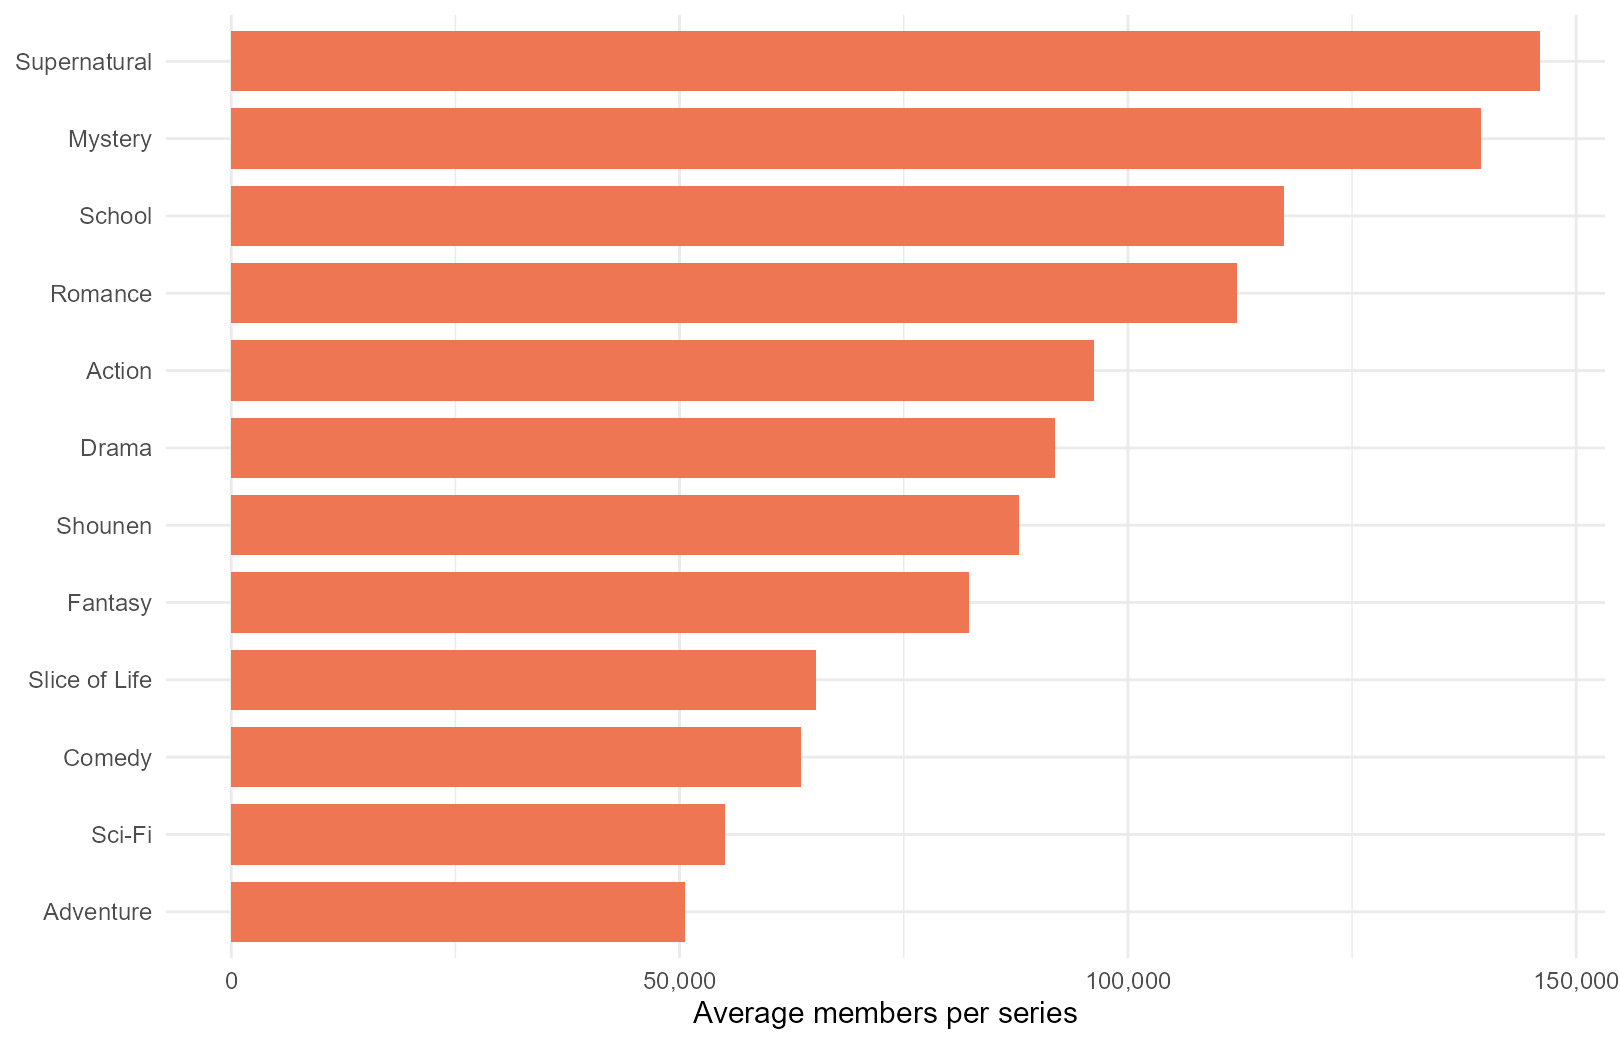
\includegraphics[width=.82\textwidth,height=.54\textheight,keepaspectratio]{generos_ranking.png}
  \end{center}
  \begin{block}{Genre Engagement Takeaway}
    Although Comedy leads in total show volume, Action, Supernatural, and
    Mystery achieve significantly higher average engagement per individual
    title.
  \end{block}
  \vspace{0.1cm}
  \centering \tiny \textit{Note: Evaluated as average members per series
  ($\text{mean}(\text{members})$) to eliminate total title volume bias
  (e.g., Comedy having many titles).}
\end{frame}

\begin{frame}{Studio Advantage \& Episode Format Strategy}
  \begin{center}
    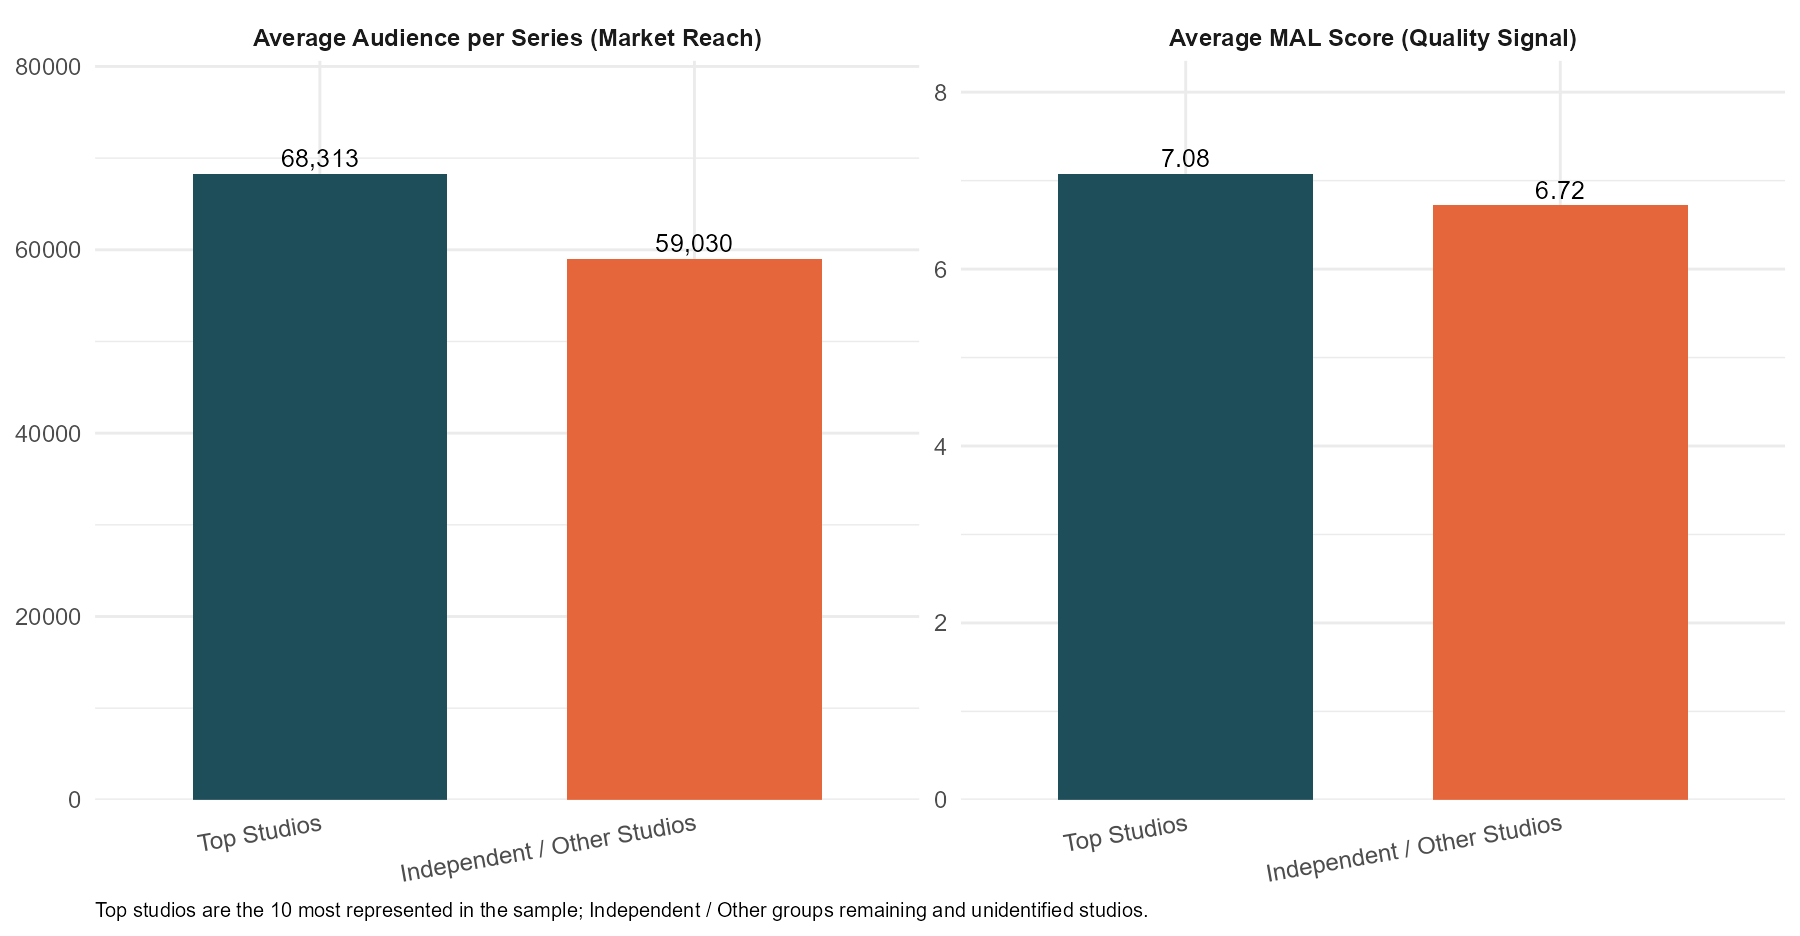
\includegraphics[width=.9\textwidth,height=.48\textheight,keepaspectratio]{top_studios_comparacion.png}
  \end{center}
  \begin{exampleblock}{Strategic Takeaway for Independent Studios}
    Concentrating capital
    in the compact 2--50 episode format avoids the high capital drain of
    long-running shows ($> 100$ eps) while maximizing audience engagement and
    ROI.
  \end{exampleblock}
  \vspace{0.1cm}
  \centering \tiny \textit{Note: Top studios average 2.11 titles per identified
  studio/year vs. 0.08 for Independent / Other, with higher scores
  (7.08 vs. 6.72); this is consistent with economies of scale rather than a
  quality-quantity trade-off. Top Studios are the 10 most represented;
  Independent / Other includes remaining and unidentified studios. Annual
  rates average over 1961--2018 and exclude unidentified studios; descriptive,
  not causal.}
\end{frame}

\begin{frame}{OLS Regression Results (HC1 Standard Errors)}
  \centering
  \resizebox{!}{.32\textheight}{
    \begin{tabular}{lrrr}
      \toprule
      \textbf{Variable} & $\mathbf{\beta}$ & \textbf{HC1 SE} & \textbf{p-value} \\
      \midrule
      Constant & -3.2048 & 0.2384 & 0.0000 \\
      Spring season & -0.0647 & 0.0670 & 0.3343 \\
      Summer season & 0.2612 & 0.0774 & 0.0007 \\
      Fall season & 0.0046 & 0.0674 & 0.9457 \\
      Sequel & 0.2692 & 0.0505 & 0.0000 \\
      Top studio & 0.1155 & 0.0482 & 0.0165 \\
      Manga source & 0.4253 & 0.0520 & 0.0000 \\
      Era 2000--2009 & 1.5135 & 0.0587 & 0.0000 \\
      Era 2010--2018 & 2.2972 & 0.0619 & 0.0000 \\
      MAL score & 1.6015 & 0.0352 & 0.0000 \\
      Episodes 51--100 & -0.6724 & 0.0700 & 0.0000 \\
      Episodes $>100$ & -0.4779 & 0.1171 & 0.0000 \\
      \bottomrule
    \end{tabular}
  }
  \vspace{0.1cm}
  \begin{block}{Notes}
    \tiny
    Estimates include genre indicators. Winter, pre-2000, and compact format
    (2--50 episodes) are the reference categories. Coefficients, HC1 standard
    errors, and p-values are reported to four decimal places, without
    significance stars. HC1 standard errors apply a finite-sample correction
    ($n/(n-k)$) for inference under heteroskedasticity.
  \end{block}
\end{frame}

\begin{frame}{Heteroskedasticity Diagnostic: Residual Scatter Plot}
  \begin{center}
    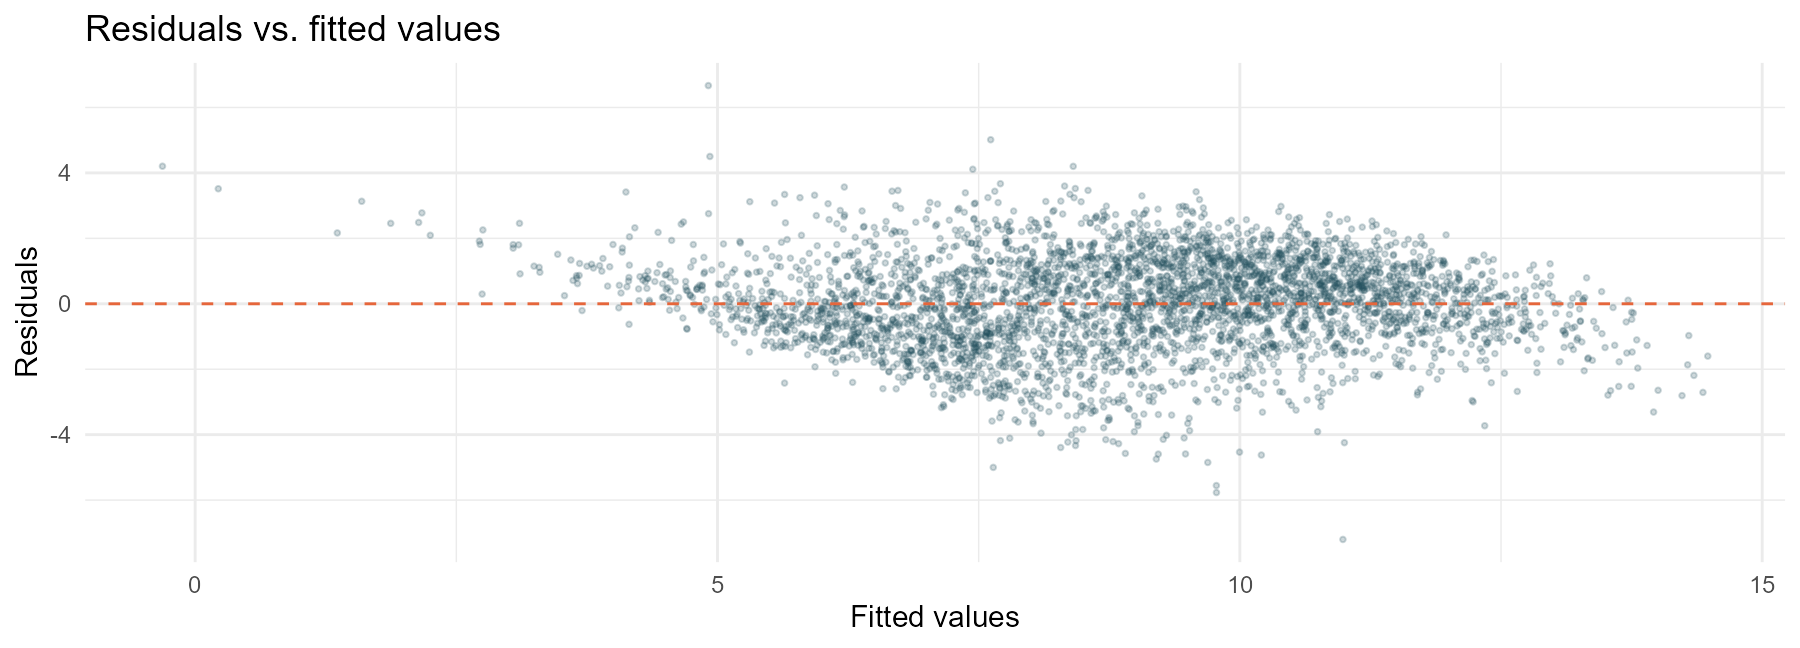
\includegraphics[width=0.80\textwidth,height=.40\textheight,keepaspectratio]{plots/residual_dispersion.png}
  \end{center}
  \vspace{-0.2cm}
  \begin{block}{Diagnostic Finding: Severe Fan-Shaped Variance}
    \footnotesize
    Residual dispersion shows a distinct funnel/fan shape as fitted values
    increase, violating constant error variance
    ($\text{Var}(\epsilon_i \vert{} X) = \sigma^2$). The Breusch--Pagan test
    confirms severe heteroskedasticity ($p < 0.0001$), formally proving that
    homoskedastic OLS inference is invalid.
  \end{block}
\end{frame}

\begin{frame}{Comparative OLS Results: Classical vs. HC1 Robust SE}
  \begin{columns}[T]
    \begin{column}{0.48\textwidth}
      \centering
      \scriptsize
      \textbf{Classical OLS (Homoskedastic)}\\[.3em]
      \resizebox{\linewidth}{!}{
        \begin{tabular}{lrrr}
          \toprule
          Variable & $\beta$ & Classical SE & $p$-value \\
          \midrule
          Constant & -3.2048 & \textcolor{red}{0.2054} & 0.0000 \\
          Spring season & -0.0647 & \textcolor{red}{0.0646} & \textcolor{red}{0.3169} \\
          Summer season & 0.2612 & \textcolor{red}{0.0766} & 0.0007 \\
          Fall season & 0.0046 & \textcolor{red}{0.0661} & \textcolor{red}{0.9447} \\
          Sequel & 0.2692 & \textcolor{red}{0.0502} & 0.0000 \\
          Top studio & 0.1155 & \textcolor{red}{0.0513} & \textcolor{red}{0.0245} \\
          Manga source & 0.4253 & \textcolor{red}{0.0529} & 0.0000 \\
          Era 2000--2009 & 1.5135 & \textcolor{red}{0.0624} & 0.0000 \\
          Era 2010--2018 & 2.2972 & \textcolor{red}{0.0626} & 0.0000 \\
          MAL score & 1.6015 & \textcolor{red}{0.0286} & 0.0000 \\
          Episodes 51--100 & -0.6724 & \textcolor{red}{0.0725} & 0.0000 \\
          Episodes $>100$ & -0.4779 & \textcolor{red}{0.1143} & 0.0000 \\
          \bottomrule
        \end{tabular}
      }
    \end{column}
    \begin{column}{0.48\textwidth}
      \centering
      \scriptsize
      \textbf{HC1 Robust OLS (Baseline)}\\[.3em]
      \resizebox{\linewidth}{!}{
        \begin{tabular}{lrrr}
          \toprule
          Variable & $\beta$ & HC1 SE & $p$-value \\
          \midrule
          Constant & -3.2048 & 0.2384 & 0.0000 \\
          Spring season & -0.0647 & 0.0670 & 0.3343 \\
          Summer season & 0.2612 & 0.0774 & 0.0007 \\
          Fall season & 0.0046 & 0.0674 & 0.9457 \\
          Sequel & 0.2692 & 0.0505 & 0.0000 \\
          Top studio & 0.1155 & 0.0482 & 0.0165 \\
          Manga source & 0.4253 & 0.0520 & 0.0000 \\
          Era 2000--2009 & 1.5135 & 0.0587 & 0.0000 \\
          Era 2010--2018 & 2.2972 & 0.0619 & 0.0000 \\
          MAL score & 1.6015 & 0.0352 & 0.0000 \\
          Episodes 51--100 & -0.6724 & 0.0700 & 0.0000 \\
          Episodes $>100$ & -0.4779 & 0.1171 & 0.0000 \\
          \bottomrule
        \end{tabular}
      }
    \end{column}
  \end{columns}
  \vspace{-.1cm}
  \begin{block}{Note}
    \tiny
    Comparing side-by-side shows that classical OLS alters standard errors
    deck-wide (underestimating uncertainty in MAL score while overestimating
    it in Top Studio), confirming why HC1 robust correction is required for
    valid inference.
  \end{block}
\end{frame}

\begin{frame}{OLS Results: Econometric Interpretation Guide}
  \begin{table}
    \centering
    \begin{tabular}{p{.23\textwidth}p{.68\textwidth}}
      \toprule
      Concept & Interpretation \\
      \midrule
      Coefficient $\beta$ & For a one-unit increase,
      $\%\Delta \mathrm{members} \approx 100\times\beta$; exact change is
      $100(\exp(\beta)-1)$. \\
      HC1 standard error & Heteroskedasticity-robust estimate of
      coefficient uncertainty with a finite-sample correction. \\
      $p$-value & Evidence against the null hypothesis that the coefficient
      equals zero. \\
      Reference category & Winter for season, pre-2000 for era, and 2--50
      episodes for format; the most frequent primary genre for genre controls. \\
      \bottomrule
    \end{tabular}
  \end{table}
\end{frame}

\begin{frame}{K-Means Results: Anime Series Profiles}
  \centering
  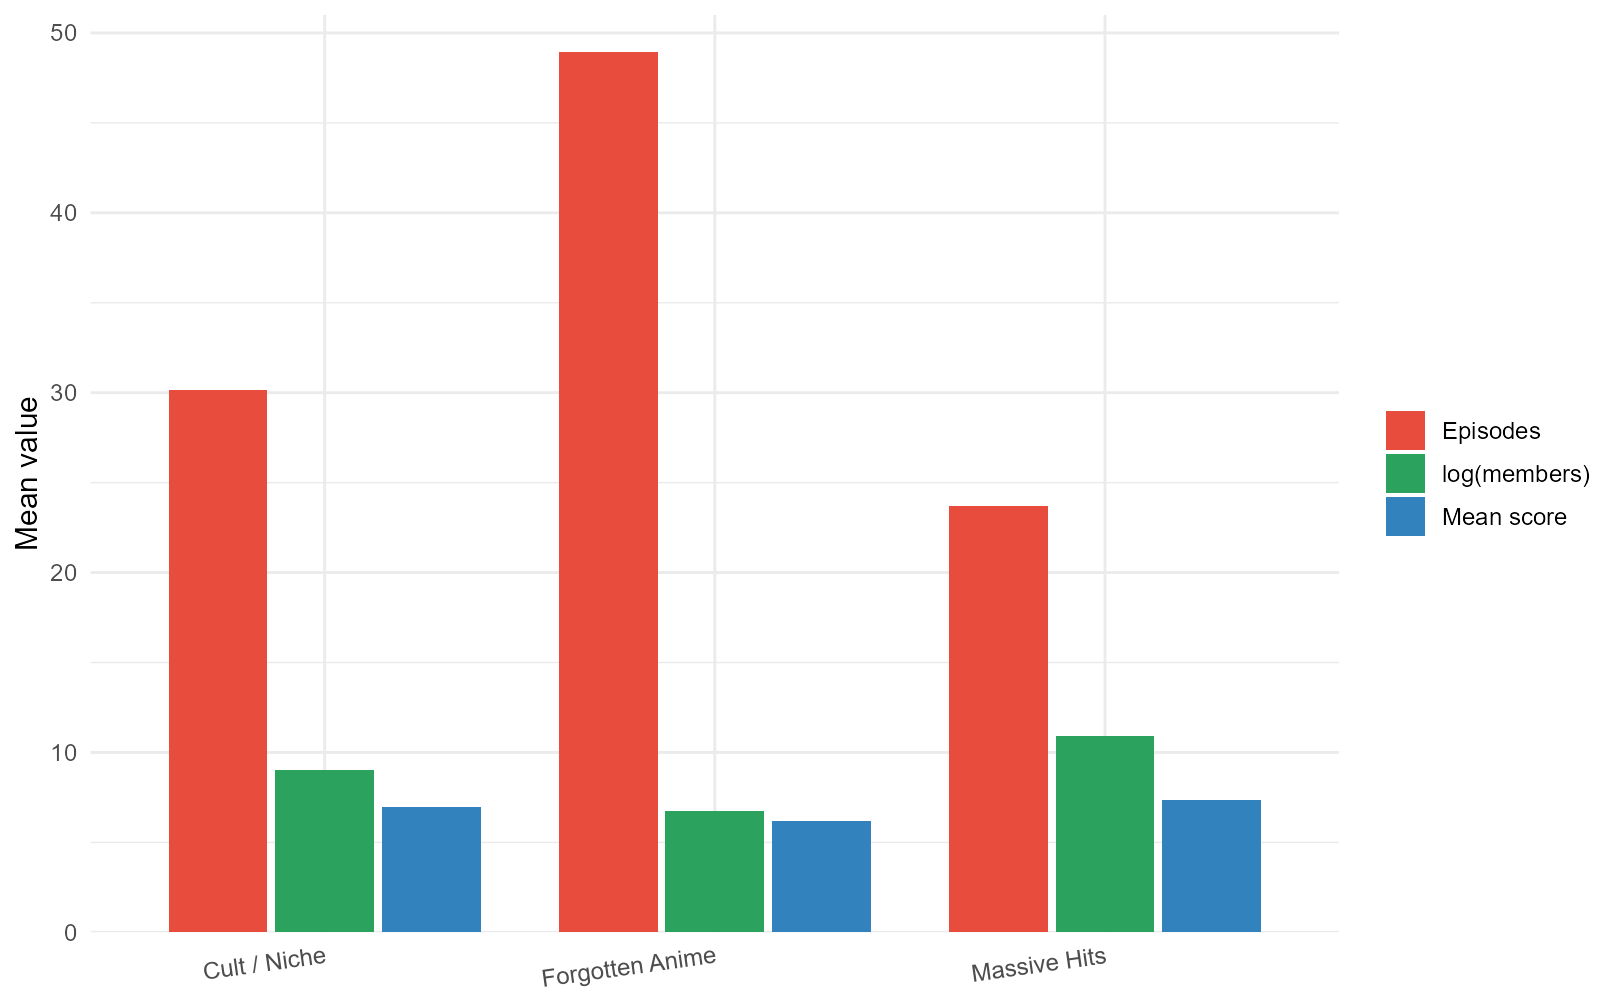
\includegraphics[width=.76\textwidth,height=.36\textheight,keepaspectratio]{kmeans_perfiles.png}
  \vspace{.2em}
  \scriptsize
  \resizebox{.86\textwidth}{!}{\begin{tabular}{lrrrr}
\toprule
Profile & N & Mean episodes & Mean log(members) & Mean score
\\
\midrule
Massive Hits & 1678 & 23.69 & 10.89 & 7.37
\\
Cult / Niche & 669 & 30.17 & 9.02 & 6.96
\\
Forgotten Anime & 1561 & 48.94 & 6.75 & 6.21
\\
\bottomrule
\end{tabular}
}
  \vspace{0.2cm}
  \begin{exampleblock}{Profile Takeaway}
    Massive hits have higher average scores and shorter episode counts.
  \end{exampleblock}
  \vfill
  {\tiny \textit{Note: Profiles are based on anime content and performance
  characteristics, not user demographic data.}}
\end{frame}

\begin{frame}{Random Forest Results: Variable Importance}
  \centering
  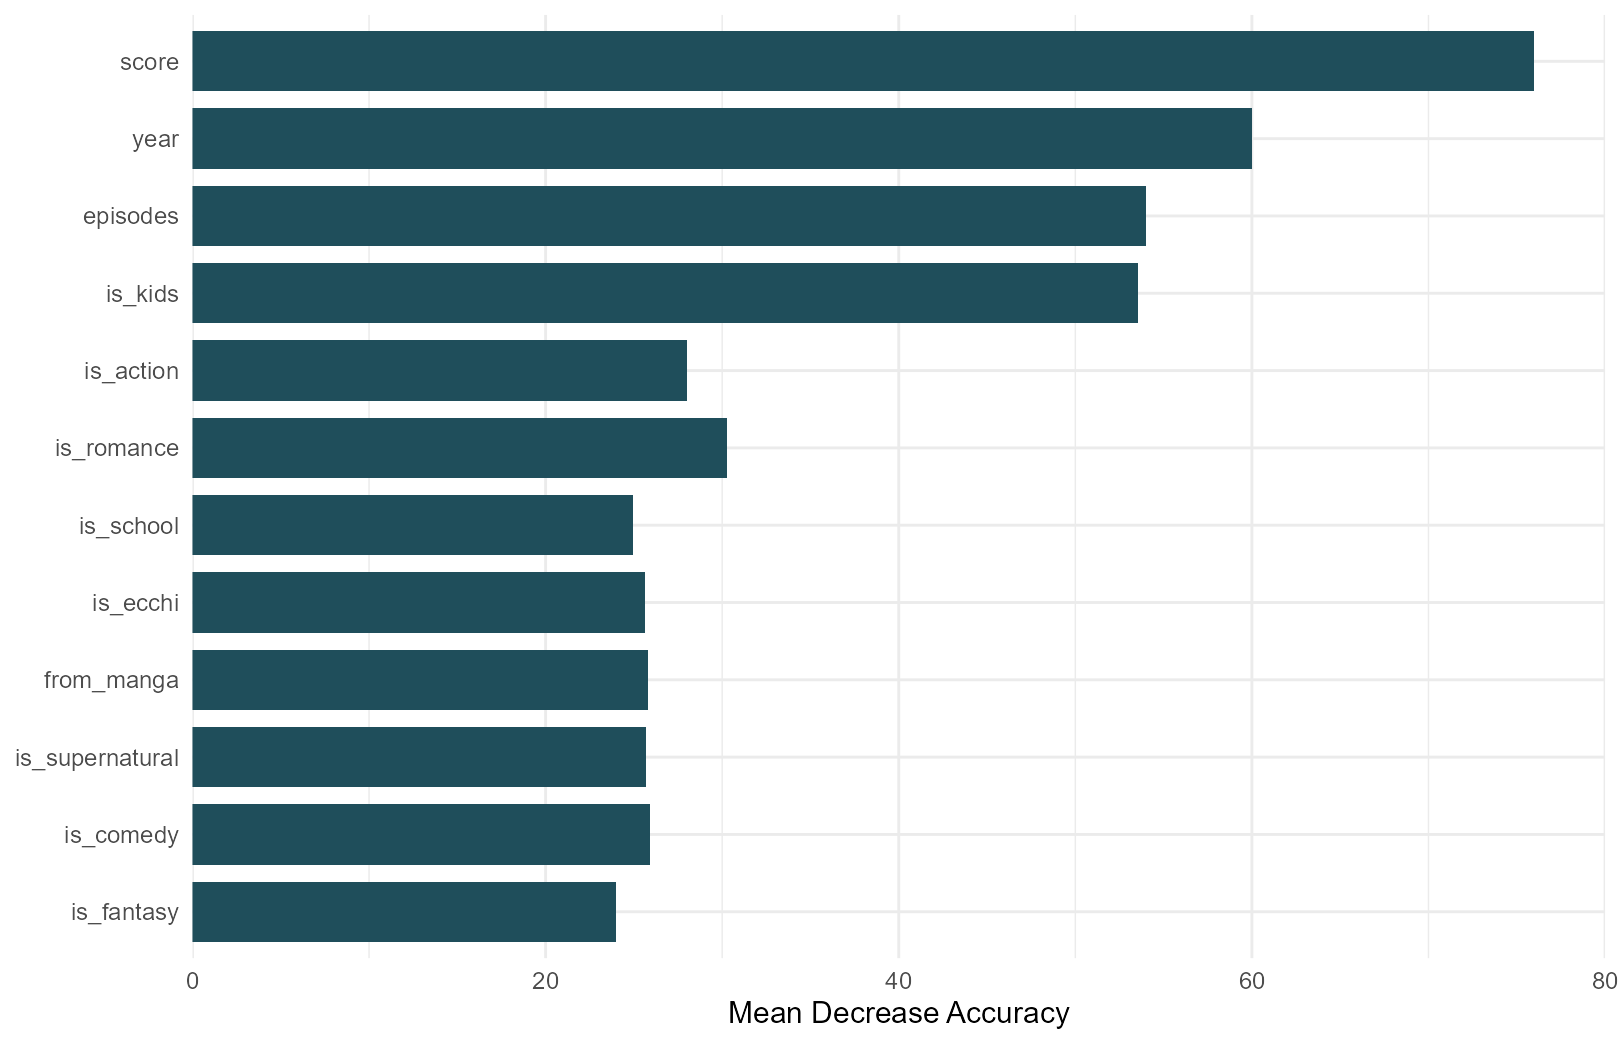
\includegraphics[width=.82\textwidth,height=.46\textheight,keepaspectratio]{rf_importancia.png}
  \vspace{.2em}
  \begin{block}{How to Read Variable Importance}
    \small Variable importance is measured by \textit{Mean Decrease Accuracy}:
    the reduction in predictive accuracy when a variable is permuted.
  \end{block}
\end{frame}

\begin{frame}{Out-of-Sample Predictive Evaluation}
  \begin{center}
    \textbf{Performance on the 20\% test set}
  \end{center}
  \vspace{.4em}
  \centering
  \begin{tabular}{lrr}
\toprule
Model & Test R-squared & Test RMSE
\\
\midrule
Random Forest & 0.836 & 1.026
\\
OLS & 0.767 & 1.221
\\
Decision Tree & 0.759 & 1.243
\\
\bottomrule
\end{tabular}

  \vspace{.6em}
  \begin{itemize}
    \item Random Forest achieves the highest predictive performance
      ($R^2 = 0.836$).
    \item OLS provides a strong, interpretable benchmark ($R^2 = 0.767$).
  \end{itemize}
\end{frame}

\begin{frame}{Conclusion \& Strategic Industry Recommendations}
  \scriptsize
  \begin{block}{Econometric Summary}
    \begin{itemize}
      \item Random Forest achieves out-of-sample $R^2 = 0.836$.
      \item MAL score, top studios, and manga source are the primary drivers
        of engagement.
    \end{itemize}
  \end{block}
  \begin{block}{Executive Production Strategy}
    \tiny
    \begin{itemize}\setlength{\itemsep}{4pt}
      \item \textbf{Prioritize compact formats (2--50 episodes):}
        Higher episode counts reduce engagement
        ($\beta = -0.6724, p < 0.001$; about $-49.0\%$); massive hits average
        around 23 episodes.
      \item \textbf{Leverage manga IP and Summer releases:}
        Manga source is associated with about $+53.0\%$ engagement
        ($\beta = 0.4253, p < 0.001$); Summer with $+29.8\%$
        ($\beta = 0.2612, p = 0.0007$).
      \item \textbf{Compete through quality and source material:}
        Top studios have a baseline advantage
        ($\beta = 0.1155, p = 0.0165$); prioritize high anime scores
        ($\beta = 1.6015$) and strong IP.
      \item \textbf{Account for streaming-era growth:}
        Engagement rose relative to pre-2000 in the 2000s
        ($\beta = 1.5135, p < 0.001$) and 2010s
        ($\beta = 2.2972, p < 0.001$).
    \end{itemize}
  \end{block}
  \begin{block}{Limitations \& Future Research}
    \tiny
    \begin{itemize}\setlength{\itemsep}{0pt}
      \item \textbf{Data Constraints:} Unobserved marketing expenditures and
        SVOD platform licensing terms.
      \item \textbf{Future Directions:} Extending cross-sectional analysis to
        panel data to track weekly viewership growth trajectories.
    \end{itemize}
  \end{block}
\end{frame}

\begin{frame}{References \& Academic Citations}
  \footnotesize
  \begin{itemize}\setlength{\itemsep}{.8em}
    \item Caves, R. E. (2000). \textit{Creative Industries: Contracts between
      Art and Commerce}. Harvard University Press.
    \item Dellarocas, C., Zhang, X. M., \& Awad, N. F. (2007). Exploring the
      value of online product reviews in forecasting sales.
      \textit{Journal of Interactive Marketing}, 21(4), 23--45.
    \item Hadida, A. L. (2010). Commercial success and artistic recognition
      in creative industries. \textit{Journal of Cultural Economics}, 34(1),
      45--67.
    \item Kim, J., et al. (2020). Machine learning applications in predicting
      digital media consumption. \textit{Empirical Economics}, 58(3),
      1120--1145.
  \end{itemize}
\end{frame}

\end{document}
